%-*-coding: utf-8-*-
\chapter{Практическая реализация и результаты}

\section{Реализация}

Предложенный подход был реализован на языке C++.  Как и в
статье~\cite{li2010practical}, было принято решение анализировать не
исходный код на C/C++, а промежуточное представление
LLVM~\cite{lattner2004llvm}. У такого подхода есть несколько весомых
преимуществ~\cite{merz2012llbmc}. Во-первых, LLVM-IR состоит из более
простых языковых конструкций, нежели C или тем более C++, что упрощает
анализ и позволяет охватить большее число возможностей языка с
меньшими усилиями. Во-вторых, код LLVM-IR представляет из себя
результат работы компилятора и является очень близким к тому, что
будет реально выполняться. Это позволяет найти ошибки, появившиеся в
результате трансформаций, выполняемых компилятором. Также
инфраструктура LLVM содержит огромное число встроенных оптимизаций,
средств для анализа и т. п., что можно использовать при
реализации. Ещё одним преимуществом анализа LLVM-IR является то, что
за счёт этого автоматически поддерживается любой язык, для которого
есть компилятор в LLVM-IR, не только C и C++ (являющиеся примерами
таких языков). Также стоит отметить, что программа в LLVM-IR всегда
представлена в SSA форме, на которой базируется описанный ранее
алгоритм. Альтернативное решение состоит в построении SSA формы для
исходной программы на C/C++ и её анализе, однако было показано, что
анализ LLVM-IR имеет существенные преимущества. Язык C++ был выбран
для реализации анализатора преимущественно по двум
причинам. Во-первых, библиотека LLVM написана на C++ и может быть
использована напрямую. Для большого числа популярных языков написаны
интерфейсы вызова сторонних функций библиотеки LLVM, однако они могут
быть неполными или устаревшими. Во-вторых, за счёт использования C++
проще достичь высокой производительности.

Изначально подход из статьи~\cite{li2010practical} был реализован в
полном соответствии с описанием. После этого было проведено
исследование работы алгоритма на различных тестовых примерах, найдены
недостатки и разработаны способы их устранения, описанные в предыдущей
главе.

\subsection{LLVM}

В LLVM каждое значение (\texttt{llvm::Value}) идентифицируется обычным
указателем (\texttt{llvm::Value *}), поэтому диапазоны переменных
ассоциируются с указателями на значения. Для идентификации инструкций
в рамках use range используются указатели на базовые блоки
(\texttt{llvm::BasicBlock}), поскольку use range переменной одинаков
во всех инструкциях из одного базового блока. Для выявления
инструкций, выделяющих блоки памяти, используется функция
\texttt{llvm::isAllocationFn}. Размер массива вычисляется как число
байт, выделяемых такой функций, поделённое на размер типа данных в
массиве. Информация о размере типа в байтах также предоставляется
LLVM. В качестве инструкций, обращающихся к памяти, рассматриваются
\texttt{store} и \texttt{load}. Анализатор начинает вычисление
диапазонов, только встретив одну из этих инструкций, то есть анализ
выполняется «по требованию».

Также LLVM предоставляет полезные функции и классы для расчёта use
range. Для проверки того, что инструкция доминируется предикатным
узлом, необходимой для уточнения use range, используется
\texttt{llvm::DominatorTree}, с помощью которого можно проверять
предикат доминируемости. Другая функциональность, необходимая для
уточнения диапазона значений, заключается в проверке достижимости
одного базового блока из другого. В общем случае такая проверка
невозможна, однако в LLVM есть функция
\texttt{llvm::isPotentiallyReachable}, которая возвращает
\texttt{false}, если базовый блок точно недостижим, и \texttt{true} в
противном случае. Как было показано в предыдущей главе, простая
проверка достижимости не является достаточно точной и может приводить
к неправильным результатам. При более точном подходе необходимо
игнорировать рёбра из $C$, кроме ребра $C \rightarrow S$. Поэтому
использовалась модифицированная версия функции, игнорирующая такие
рёбра.

При обнаружении ошибки о ней необходимо сообщить пользователю в
понятном формате. Для этого нужно сопоставлять инструкции из
промежуточного представления LLVM выражениям в исходном коде на
высокоуровневом языке. Эта проблема решается за счёт использования
отладочной информации, генерируемой компилятором при использовании
специального флага. В LLVM такая информация представлена классом
\texttt{DebugLoc}. Если программа скомпилирована с отладочной информацией, то
по инструкции LLVM можно получить её \texttt{DebugLoc} и сообщить
пользователю, где в исходном коде находится ошибка.

\subsection{Gated Single Assignment}

Одной из наиболее важных деталей алгоритма является использование
Gated Single Assignment формы
(GSA)~\cite{ottenstein1990program}. Отличие этой формы от SSA
заключается в том, что аргументы $\phi$-инструкций также содержат
условия, которые гарантировано выполняются, если данное значение
возвращается $\phi$-инструкцией. Это позволяет существенно повысить
точность анализа, отбрасывая невозможные значения переменных.

В реализации анализатора использовался алгоритм для конвертации SSA
формы в GSA, описанный в статье~\cite{tu1995efficient}. Данный
алгоритм является одним из наиболее простых в реализации. Он не
требует, чтобы исходная программа была в SSA, однако существенно
упрощается, если это выполнено. В основе алгоритма лежит понятие
«выражение пути» (path expression), которое является регулярным
выражением над алфавитом, состоящим из рёбер в графе потока
управления. Пути, приходящие в $\phi$-инструкцию, представляются
выражениями пути. В конце работы алгоритма выражения пути превращаются
в предикаты GSA-формы. Несмотря на свою простоту, алгоритм также
является более эффективным по сравнению со своими аналогами. В
результате работы алгоритма для каждого операнда каждой
$\phi$-инструкции известен определённый набор условий, который должны
выполняться, чтобы данное значение было результатом
$\phi$-инструкции. После этого вычисленные условия применяются для
уточнения диапазонов значений $\phi$-инструкций в месте их определения.

\subsection{Символьные вычисления}

Базовой составляющей алгоритма являются символьные вычисления,
используемые для расчёта диапазонов значений переменных в программе. В
статье~\cite{li2010practical} используются три понятия для описания
символьных вычислений: символы-атомы, символьные выражения и
символьные диапазоны. Изначально множество символов-атомов пустое,
однако оно пополняется в ходе анализа. Это происходит, когда результат
какой-то операции не может быть представлен афинной функцией
существующих символов-атомов. В этом случае добавляются новые
символы-атомы, являющиеся афинными преобразованиями существующих
атомов. Символьные выражения являются афинными преобразованиями
символов-атомов. Символьные диапазоны представляются парой символьных
выражений.

Для представления символов-атомов используются четыре класса:
\texttt{atomic\_const, atomic\_var, atomic\_linear,
  atomic\_bin\_op}. \texttt{atomic\_const} соответствует константному
атому и хранит одно число. \texttt{atomic\_var} соответствует
некоторому значению в программе и хранит указатель на это значение
(являющееся идентификатором). \texttt{atomic\_linear} используется для
представления атома, являющегося произведением другого атома и
константы. Наконец, \texttt{atomic\_bin\_op} представляет применение
простейшей бинарной операции к двум атомам. С помощью этих классов
можно представить любой символ-атом, т. к. он задаётся как афинное
преобразование других символов-атомов. Нетрудно видеть, что
\texttt{atomic\_linear} может быть представлен как
\texttt{atomic\_bin\_op} с операцией умножения, однако за счёт выделения
\texttt{atomic\_linear} в отдельный класс упрощается распознание
предикатов, используемых для учёта зависимостей потока управления.

Символьное выражение представляется классом \texttt{sym\_expr}, внутри
которого хранятся два числа \texttt{coeff} и \texttt{delta} и
символ-атом \texttt{atom}. Такое представление соответствует
символьному выражению, являющемуся афинным преобразованием атома
\texttt{atom}: \texttt{coeff $\cdot$ atom + delta}. Помимо этого
внутри \texttt{sym\_expr} хранится специальный флаг
(\texttt{boost::tribool}), для задания $\bot$ и $\top$. Флаг может
принимать три значения, два из которых соответствуют $\bot$ и $\top$,
а третье соответствует обычному символьному выражению. Всего в
программе существует ровно один $\bot$ и ровно один $\top$. Для
символьных выражений определены операции сложения, вычитания,
умножения, деления, проверка равенства и неравенства и сравнение путём
перегрузки операторов. Определения этих операций соответствуют
описанию из статьи~\cite{li2010practical}. Наибольшую трудность
представляют операции умножения и деления, так как для них необходимо
рассматривать большое число частных случаев, например, когда какой-то
коэффициент равен нулю. Помимо этого определены операции \texttt{meet}
и \texttt{join}.

Последней сущностью, используемой для символьных вычислений, является
символьный диапазон. Для его представления используется простая
структура \texttt{sym\_range}, состоящая из двух полей типа
\texttt{sym\_expr}. Для удобства определяются два специальных
диапазона: \texttt{empty} и \texttt{full}, соответствующие пустому
диапазону ($[\top, \bot]$) и диапазону, содержащему любой другой
диапазон ($[\bot, \top]$). Операции сложения, умножения, вычитания
деления определены как для пары диапазонов, так и для пары из
диапазона и выражения. Также определены операции пересечения и
объединения двух диапазонов.

\subsection{Обработка больших программ}

Одной из главных проблем при обработке больших программ, состоящих из
большого числа файлов и сложного механизма сборки, является
необходимость скомпилировать программу в LLVM-IR. Для решения проблемы
используется утилита \texttt{whole-program-llvm}~\cite{wllvm},
написанная на языке Python, которая используется также в проекте
KLEE~\cite{cadar2008klee}. Утилита подменяет компилятор (\texttt{gcc}
или \texttt{clang}) обёртками, которые помимо компиляции кода также
сохраняют дополнительную служебную информацию о расположении кода в
генерируемых файлах. При линковке объектных файлов служебная
информация объединяется. Таким образом, получающийся в результате
сборки исполняемый файл (или библиотека) содержит всю необходимую
информацию для восстановления биткода. На последнем шаге из файла
извлекается биткод, соответствующий всей программе целиком. При этом
сохраняется отладочная информация, если она была сгенерирована
компилятором. В дальнейшем биткод полностью передаётся
анализатору. Поскольку утилита является простой обёрткой над
компилятором, её очень легко использовать с различными системами
сборки, такими как \texttt{GNU Make}~\cite{gnumake}. Достаточно лишь
верно указать используемый компилятор, чтобы обычно делается с помощью
переменных окружения. Также были написаны небольшие скрипты для
автоматизации стандартного процесса анализа: компиляция программы с
помощью \texttt{wllvm}, извлечение биткода, запуск анализатора.

\section{Экспериментальные результаты}

После реализации анализатора были проведены различные исследования для
оценки получившихся результатов.

\subsection{Результаты использования анализатора}

Для проверки работоспособности и эффективности разработанного
анализатора было произведено его тестирование на крупных open-source
проектах. В рамках тестирования были проанализированы система сборки
CMake версии 3.1.0 и игра Multi Theft Auto версии 1.3.1. Оба проекта
состоят из сотен тысяч строчек кода как на C, так и на C++.

CMake содержит 180000 строчек кода на C++ и 170000 строчек кода на
C. После компиляции в LLVM размер биткода составил 31
мегабайт. Обработка заняла чуть больше одиннадцати минут. Анализатор
запускался в режиме, в котором спорные ситуации пропускаются. В таком
режиме было найдено восемь ошибок. Найденные ошибки были проверены
вручную, в результате оказалось, что пять из них являются реальными
ошибками, а остальные три являются ложными срабатываниями. В новых
версиях CMake ошибки были исправлены, что подтверждает факт ошибок.

Multi Theft Auto содержит 410000 строчек кода на C++ и 350000 строчек
кода на C. Размер биткода составил 182 мегабайта. Обработка заняла
немногим более сорока минут, что в целом приемлемо для столь большого
проекта. Вновь использовался режим, в котором спорные ситуации
пропускаются. Всего было найдено одиннадцать ошибок. В результате
ручной проверки семь из них оказались действительными ошибками. Ещё
четыре ошибки были обнаружены неверно.

\begin{table}[!h]
\caption{Результаты работы анализатора}\label{tab:analyzer-results}
\centering
  \begin{tabular}{|*{18}{c|}}\hline
  Программа   & Строки кода & Биткод & Время & Общее число & TP & FP \\\hline
  CMake 3.1.0 & 350000      & 31M    & 11:03 & 8           & 5  & 3  \\\hline
  MTA 1.3.1   & 760000      & 182M   & 42:49 & 11          & 7  & 4  \\\hline
  \end{tabular}
\end{table}

В таблице~\ref{tab:analyzer-results} подведены итоги экспериментальных
запусков. Вторая колонка содержит число строк кода, третья колонка
показывает размер биткода, полученного в результате
компиляции. Следующая колонка содержит время работы
анализатора. Наконец, последние три колонки содержат общее число
найденных ошибок, число верно найденных ошибок (в таблицах
обозначается как TP, true positive) и число ложных срабатываний (в
таблицах обозначается как FP, false positive). Таким образом,
разработанное средство статического анализа действительно способно
обрабатывать программы большого размера за разумное время и находить в
них ошибки. К сожалению, число ложных срабатываний оказалось
сопоставимо с числом реальных ошибок, поскольку было сделано большое
число упрощений с целью повышения скорости работы. Однако в целом
число ложных срабатываний невелико, и ручная проверка занимает
довольно мало времени. Во многих ситуациях способность находить
реальные ошибки является более важной, чем необходимость потратить
немного времени на ручной анализ.

\subsection{Сравнение с другими анализаторами}

Также было проведено сравнение разработанного анализатора с другими
доступными анализаторами C/C++ кода. Использовались следующие
анализаторы: Cppcheck, PVS-Studio, Splint, LLBMC, а
также реализация анализатора, описанного в
статье~\cite{li2010practical}, и реализация предложенного подхода. В
первой главе присутствует краткое описание каждого
анализатора. Cppcheck запускался с аргументами \texttt{--std=c++11
  --std=c11 --enable=warning --inconclusive}, из найденных ошибок
выбирались содержащие фразу \texttt{out of bounds}, соответствующие
выходу за пределы массива. PVS-Studio запускался со стандартными
настройками, рассматривались ошибки V557 (выход за пределы
массива). Splint запускался с флагами \texttt{-weak -hints
  +bounds}. Утилита LLBMC, к сожалению, распространяется лишь в
бинарном формате и не обновлялась уже много лет, в связи с чем
поддерживает лишь очень старую версию LLVM, поэтому произвести анализ
с её помощью не удалось.

Сравнение проводилось на Multi Theft Auto 1.3.1 и CMake 3.1.0,
упомянутых ранее, а также на наборе синтетических тестов,
представленных в листинге~\ref{lst:comparison}.

\begin{table}[!h]
\caption{Сравнение анализаторов: Multi Theft Auto 1.3.1}\label{tab:comparison-mta}
\centering
  \begin{tabular}{|*{18}{c|}}\hline
  --                 & TP  & FP  & Время работы \\\hline
  Cppcheck           & 1   & 8   & 11:53        \\\hline
  PVS-Studio         & 4   & 0   & 10:36        \\\hline
  Splint             & --- & --- & ---          \\\hline
  LLBMC              & --- & --- & ---          \\\hline
  Li et at.          & 7   & 202 & 37:55        \\\hline
  Предложенный метод & 7   & 4   & 42:49        \\\hline
  \end{tabular}
\end{table}

Результаты сравнения на Multi Theft Auto 1.3.1 представлены в
таблице~\ref{tab:comparison-mta}. Анализаторы Cppcheck и PVS-Studio
вновь показали довольно хорошее время работы, на сей раз оно составило
немногим более десяти минут. Cppcheck смог найти лишь одну ошибку, при
этом было восемь ложных срабатываний из-за проблем с обработкой
директив препроцессора. PVS-Studio удалось найти четыре реальных
ошибки, причём снова без единого ложного срабатывания. С анализаторами
Splint и LLBMC возникли те же проблемы, что и для CMake, поэтому
результаты их работы собрать не получилось. Реализованный в рамках
данной работы анализатор нашёл на три ошибки больше, чем
PVS-Studio. Вновь не обошлось без небольшого числа неверно найденных
ошибок, что в целом не критично для практического использования. Время
работы оказалось сильно больше, чем у PVS-Studio и Cppcheck, однако
вполне примемлемо для проекта, содержащего почти миллион строчек
кода. Также была протестирована реализация алгоритма из
статьи~\cite{li2010practical}. Она нашла те же семь реальных ошибок,
но суммарное число найденных ошибок оказалось больше двухсот. Учитывая
проделанные изменения, можно сделать вывод, что, скорее всего, все
остальные ошибки являются недействительными. Ручная проверка всех
сообщений об ошибках, найденных этой реализацией, не проводилась ввиду
большого числа таких сообщений.

\begin{figure}
    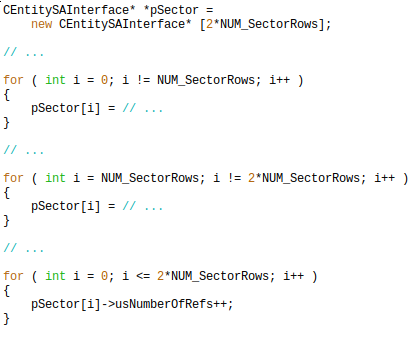
\includegraphics[]{mta-bug.png}
    \caption{Ошибка в Multi Theft Auto}
    \label{fig:mta-bug}
\end{figure}

На рисунке~\ref{fig:mta-bug} продемонстрирована упрощённая версия кода
одной из ошибок, найденных в Multi Theft Auto 1.3.1, которую не
удалось найти с помощью Cppcheck или PVS-Studio. Как видно, переменная
\texttt{pSector} указывает на массив размера \texttt{2 *
  NUM\_SectorRows}. При этом значение \texttt{NUM\_SectorRows} заранее
не известно. Сначала заполняется первая половина массива, затем
вторая. При заполнении массива все обращения к нему корректны. Однако
после этого происходит проход по всему массиву, в котором есть ошибка:
в качестве условия выхода из цикла используется предикат $\leq$, хотя
должен использоваться предикат $<$ или $!=$. Причина, по которой ни
PVS-Studio, ни Cppcheck не смогли найти такую ошибку, заключается,
по-видимому, в том, что размер массива, а также ограничение на
значение счётчика цикла, не выражаются константой или какой-то
переменной. В данном случае размер массива представляется
произведением константы и переменной. В то же время подход из
статьи~\cite{li2010practical} учитывает зависимости от переменных,
выражаемые афинными преобразованиями, за счёт чего такая ошибка
находится анализатором.

\begin{table}[!h]
\caption{Сравнение анализаторов: CMake 3.1.0}\label{tab:comparison-cmake}
\centering
  \begin{tabular}{|*{18}{c|}}\hline
  --                 & TP  & FP  & Время работы \\\hline
  Cppcheck           & 1   & 0   & 5:59         \\\hline
  PVS-Studio         & 1   & 0   & 5:18         \\\hline
  Splint             & --- & --- & ---          \\\hline
  LLBMC              & --- & --- & ---          \\\hline
  Li et at.          & 5   & 79  & 9:12         \\\hline
  Предложенный метод & 5   & 3   & 11:03        \\\hline
  \end{tabular}
\end{table}

Результаты сравнения на CMake 3.1.0 представлены в
таблице~\ref{tab:comparison-cmake}. Анализаторы Cppcheck и PVS-Studio
нашли по одной ошибке c абсолютной точностью. Причём были найдены
разные ошибки. Время работы обоих анализаторов составило менее шести
минут. Splint умеет обрабатывать только код на языке C, однако даже
при попытке запуска только на C файлах он не мог обработать многие из
них из-за ошибок, связанных с препроцессором. Как сообщалось ранее,
провести анализ утилитой LLBMC не удалось, поскольку её исходный код
отсутствует в публичном доступе а исполняемые файлы сильно
устарели. Разработанный в рамках данной работы анализатор нашёл пять
ошибок с тремя ложными срабатываниями. В то же время реализация
алгоритма из статьи~\cite{li2010practical} без модификаций нашла те же
пять ошибок, но при этом суммарное число сообщений об ошибках было
близко к сотне. Таким образом, разработанный анализатор способен
находить больше ошибок, чем существующие анализаторы. Вместе с
увеличением числа находимых реальных ошибок увеличилось и число ложных
срабатываний, а также время работы. Однако оба показателя являются
вполне приемлемыми.

\begin{table}[!h]
\caption{Сравнение анализаторов: синтетические тесты}\label{tab:comparison-synthetic}
\centering
  \begin{tabular}{|*{18}{c|}}\hline
  --                       & TP  & FP & FN \\\hline
  scan-build               & 0   & 0  & 0  \\\hline
  CppCheck                 & 3   & 0  & 9  \\\hline
  PVS-Studio               & 4   & 0  & 8  \\\hline
  Splint                   & 9   & 3  & 3  \\\hline
  LLBMC                    & -   & -  & -  \\\hline
  Li et at.                & 12  & 8  & 0  \\\hline
  Разработанный анализатор & 12  & 0  & 0  \\\hline
  \end{tabular}
\end{table}

В таблице~\ref{tab:comparison-synthetic} представлены результаты
сравнения на синтетических тестах (листинг~\ref{lst:comparison}). Этот
набор тестов содержит различные конструкции, которые нередко можно
встретить в коде: условные переходы, некоторые виды циклов, а также
тесты, в которых необходим межпроцедурный анализ. Для сравнения также
использовался статический анализатор, поставляемый с компилятором
\texttt{clang}: \texttt{scan-build}~\cite{scan-build}. Однако, как
видно из таблицы, анализатор не смог найти ни одной ошибки. Хотя
авторы заявляют наличие анализа выходов за пределы массива, работает
он лишь в совсем тривиальных случаях. Анализаторы Cppcheck и
PVS-Studio снова продемонстрировали схожие результаты и нашли 3 и 4
ошибки соответственно. Вновь не было ни единого ложного
срабатывания. Однако суммарно в тестах было 12 ошибок, поэтому число
ненайденных ошибок (False Negative, FN) весьма велико. Splint
использует другую стратегию и сообщает об ошибке всегда, когда не
может доказать её отсутствие (то есть корректность обращения к
массиву). Ему удалось найти 9 реальных ошибок, при этом было 3 ложных
срабатывания. 3 ошибки оказались не найдены. Результаты были бы лучше,
если бы Splint выполнял межпроцедурный анализ. Алгоритм, описанный
в~\cite{li2010practical} и реализованный без модификаций, нашёл все 12
реальных ошибок, однако также выдал 8 несуществующих ошибок. Наконец,
улучшенной версии анализатора, реализованной в данной работе, удалось
найти также все 12 ошибок, но без единого ложного срабатывания.

\chapterconclusion

В данной главе были описаны основные детали реализации
анализатора. Обосновано решение проводить анализ на уровне
промежуточного представления LLVM.  Приведены экспериментальные
результаты запуска анализатора на крупных проектах. Показано, что
анализатор способен находить в них ошибки, работая за приемлемое
время. Также было проведено сравнение с доступными статическими
анализаторами C/C++ кода на тех же проектах и на наборе синтетических
тестов, представленных в
листинге~\ref{lst:comparison}. Продемонстрировано, что в целом
анализатор не уступает существующим решениям и в некоторых случаях
превосходит их.
